\section{Prolegomena}\label{sec:prolegomena}

This section sets out the idea behind the paper and fixes its terms.  It contains no theorem.

\subsection{Rays on a cube, and the rule}\label{sec:rule}

Take first a ray with real coordinates: a straight line through a fixed point~$O$, with a
direction but no length and no sense.  Put $O$ at the centre of a cube that reaches from $-x$
to $x$ along three perpendicular axes, with $x>0$.  The ray leaves the cube at a point $P$ and
at the opposite point, and either names it.  A ray is a triple of numbers taken up to a common
factor.  Choose the factor so that the coordinate of largest size has size~$x$: the triple is
then~$P$, and its coordinates are read off the face on which $P$ lies.  (Rays with complex
coordinates have no such picture.)

Three mutually orthogonal rays form a \emph{triad}.  The rule is:

\begin{quote}
In every triad exactly one ray is \emph{colored}.  Two orthogonal rays are never both colored.
\end{quote}

A ray that is not colored is \emph{uncolored}.  To \emph{color a set} of rays is to decide, for
every ray in it, whether it is colored or uncolored, in agreement with the rule.  For a finite
set the rule is applied to the orthogonal pairs and the triads found within the set, and to no
others.  Two orthogonal rays of the set belong to a triad of space whose third ray may be
absent from the set, and they are forbidden to be both colored all the same.

The rule is a prediction of quantum mechanics.  For a particle of spin one, the squares of the
spin along three mutually orthogonal directions can be measured together.  Each is 0 or~1 (in
units of $\hbar^2$) and the three add up to~2, so exactly one is~0, and that direction is the
one colored.  Values fixed before the measurement, and independent of which two other
directions are measured, would color every ray in agreement with the rule.  Kochen and
Specker~\cite{KochenSpecker1967} showed that there are finite sets of rays that cannot be
colored.  Such a set is \emph{uncolorable}, or a \emph{Kochen--Specker (KS) set}.

\subsection{The grid}\label{sec:grid}

Peres drew his set of 33 rays as points on a cube, and the 31 rays of Conway and Kochen the
same way~\cite{Peres1991,Peres1993}.  In both drawings the points lie where five lines in one
direction cross five in the other.  In the first the lines sit at $0$, $\pm1$ and $\pm\sqrt2$,
in the second at $0$, $\pm1$ and~$\pm2$.  The two sets are built on \emph{the same grid},
except for the position of one pair of lines.  Write that position as~$x$
(Fig.~\ref{fig:generic}).

\begin{figure}[t]
\centering
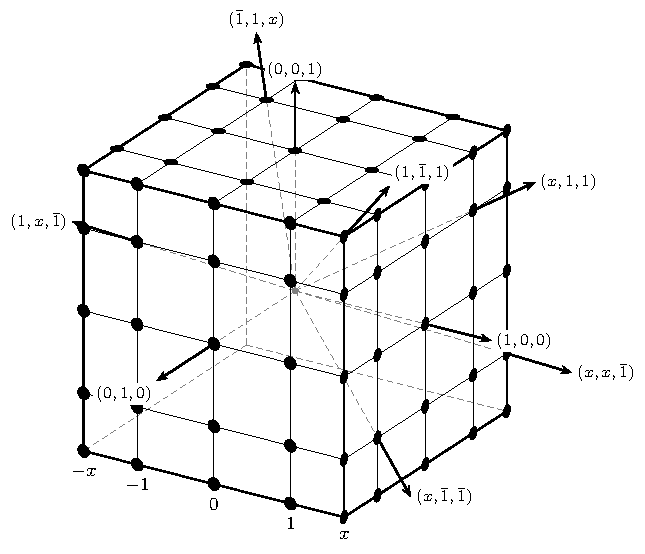
\includegraphics[width=0.5\textwidth]{figures/alphabet_cube_generic.pdf}
\caption{Coordinate triples as rays, for real $x>1$.  The cube reaches from $-x$ to $x$ on each
axis and the lines on its faces sit at $0,\pm1,\pm x$.  A bar is a minus sign.  Triples written
without~$x$, such as $(1,0,0)$ and $(1,\bar1,1)$, reach the surface after scaling by~$x$.  The
49 rays are named by the same coordinate triples for every such~$x$; which pairs are orthogonal
depends on~$x$.}
\label{fig:generic}
\end{figure}

The numbers at which the lines sit are the \emph{coordinate values}.  A \emph{coordinate
triple} is a triple of coordinate values, not all zero, such as $(x,1,\bar1)$, where a bar is a
minus sign.  Every coordinate triple names a ray, and proportional triples name the same ray.
The \emph{grid} is the set of rays so named.  Where a coordinate value is a parameter, as $x$
is here, a coordinate triple is an expression in the parameter, to be evaluated at each value
of it, and ``the same triple'' at two values of $x$ means the same expression.  For real $x>1$
the coordinate values $0,\pm1,\pm x$ give 124 coordinate triples, and they name 49 rays.  Each
of the 49 leaves the cube at a point where the lines cross, and every such point is one of the
49: the drawing is the grid.  (For other real or complex $x$ the triples again name 49 rays,
except at a few values such as $x=1$, where fewer remain.)

The same terms are used for any finite list of numbers that contains~$0$, real or complex.  In
counting coordinate values we leave out $0$ and take a value and its negative as one, so the
grid above has two coordinate values, $1$ and~$x$.  If there is a nonzero coordinate value, one
can be taken to be~$1$, since a common factor does not change a ray.

Two orthogonal rays fix a third, the ray orthogonal to both, and it need not belong to the
grid.  With coordinate values $0,\pm1,\pm2$ the triples $(1,1,2)$ and $(2,0,\bar1)$ are
orthogonal, and the ray orthogonal to both is $(1,\bar5,2)$, which no coordinate triple names.
The \emph{completed grid} is the smallest set of rays that contains the grid and contains,
with every two orthogonal rays, the third ray of their triad.  A grid and its completed grid
need not be equal, and every count in this paper says which is meant.

Earlier versions of this paper, and the programs that accompany it, use other names.  There
the list of coordinate values is an \emph{alphabet}, a coordinate value is a \emph{letter} or
\emph{symbol}, a coordinate triple is a \emph{word}, a grid is a \emph{pool} or \emph{raw
pool}, and a completed grid is a \emph{completed pool}.

\subsection{The question}\label{sec:ladder}

The coordinate triples, as expressions, do not change with~$x$.  What changes is which rays
are orthogonal.  For real~$x$,
\[
(x,1,1)\cdot(x,\bar1,\bar1)=x^2-2 ,\qquad (1,\bar1,1)\cdot(x,1,\bar1)=x-2 ,
\]
so the first pair is orthogonal only when the lines sit at $\pm\sqrt2$ and the second only
when $x=2$.  The picture shows where the rays are; it does not show which are orthogonal, and
that has to be computed.  Every such product is a sum of at most three terms, each a product
of two coordinate values.  It is zero for every~$x$, or it is one of finitely many equations
for~$x$; Table~\ref{tab:zerosums} lists, up to the symmetries stated there, those with a
solution other than $0$ and~$\pm1$.  The question of this paper is:

\begin{quote}
For which coordinate values can the grid not be colored, and how few of its rays are then
needed?
\end{quote}

\begin{figure}[t]
\centering
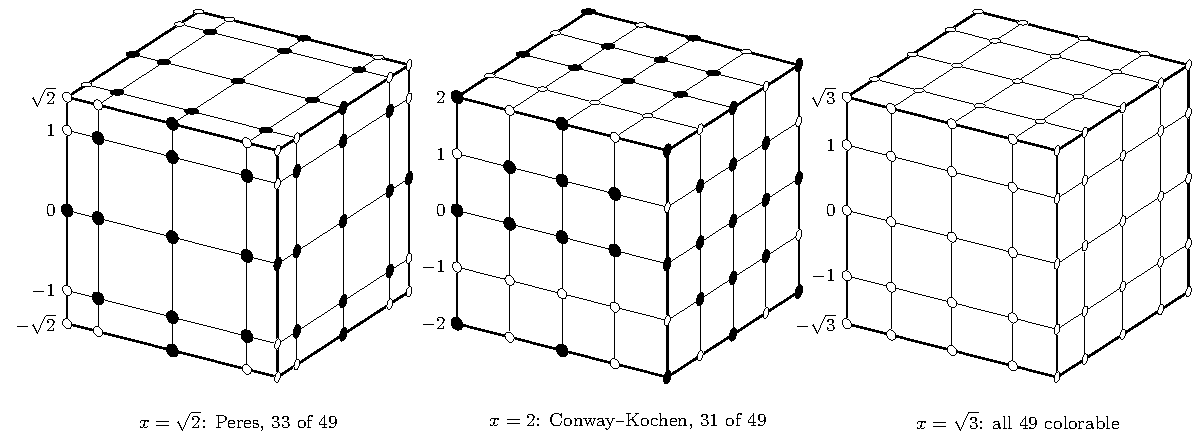
\includegraphics[width=\textwidth]{figures/alphabet_cube_triptych.pdf}
\caption{One grid at three positions of its inner lines.  Each of the 49 rays leaves the centre
of the cube through a point where the lines cross; opposite points are the same ray.  Filled
points: the 33 rays of Peres at $x=\sqrt2$ and the 31 rays of Conway and Kochen at $x=2$.  At
$x=\sqrt3$ the whole grid of 49 rays has a coloring.  Only the two inner lines move with~$x$.
The three cubes are the points \textit{A}, \textit{B} and \textit{C} of Fig.~\ref{fig:circle}.}
\label{fig:triptych}
\end{figure}

\begin{figure}[t]
\centering
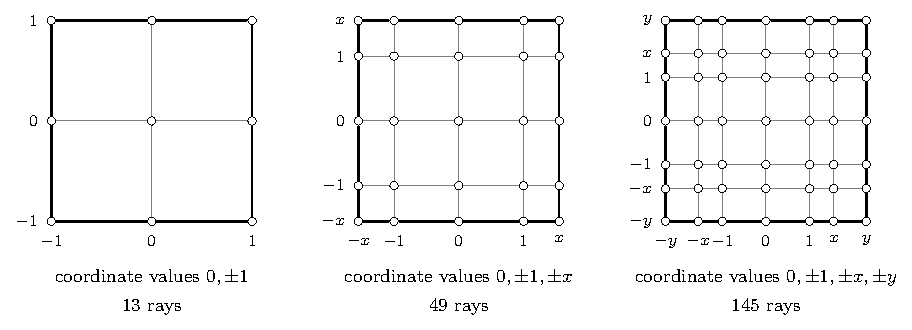
\includegraphics[width=0.84\textwidth]{figures/fig7_ladder.pdf}
\caption{Grids with one, two and three coordinate values.  One face of each cube is shown, with
lines at the coordinate values; the number of rays is that of the grid.  In the first two the
points where the lines cross, taken over all six faces with opposite points counted once, are
all the rays of the grid.  In the third they are 109 rays, and the grid has in general 145.}
\label{fig:ladder}
\end{figure}

Grids are ordered by the number of their coordinate values (Fig.~\ref{fig:ladder}, which shows
real ones).  With one, the grid has 13 rays and a coloring.  With two, $1$ and a real $x>1$, it
is the 49-ray grid of the two classical sets.  With three real ones, $1<x<y$, it has in general
145 rays, and the drawing is
no longer the whole grid: on the cube that reaches to~$y$ the ray $(1,x,0)$
leaves at $(y/x,\,y,\,0)$, which is in general not a point where lines cross, and the crossings
on the six faces are 109 rays of the 145.  A grid that lacks some of the minus signs is a
subset of one of these.  Its coloring is a separate matter, but a KS set on it is a KS set on
the larger grid.

The smallest KS set known in three dimensions has 31 rays and lies on a grid with two
coordinate values; all that is proved in general is that at least 24 rays are
needed~\cite{KirchwegerPeitlSzeider2023,LiBrightGanesh2024}.  \emph{This paper does not prove
that 31 is the minimum.}  Every finite set of rays lies on some grid if enough coordinate
values are allowed, so the classifications below exclude a smaller set only from the families
they cover: grids with two coordinate values (Theorem~\ref{thm:twosymbol}) and real grids with
three (Theorem~\ref{thm:threesymbol}).  These statements are about grids, not completed grids.
